%%%%%%%%%% the following setup maximizes number of characters per page---
%%%%%%%%%% good for solution sets, etc.  Don't use for articles.

\documentclass{amsart}
\raggedbottom
\oddsidemargin=0in
\evensidemargin=0in
\textwidth=6.5in
\textheight=9in
\topmargin=0in
\headheight=0in
\headsep=0in
\footskip=0in
\parskip=10bp
\parindent=0bp
%\footheight=0in
\pagestyle{empty}
\usepackage{amsfonts,amssymb}
\usepackage[dvips]{graphicx}

\newtheorem{defn}{Definition}

\newcommand{\BS}{\blacksquare}
\newcommand{\ini}{\mathop{\rm in}\nolimits}
\newcommand{\Proj}{\mathop{\rm Proj}\nolimits}
\newcommand{\Hilb}{\mathop{\rm Hilb}\nolimits}
\newcommand{\fld}{{\bf k}}
\newcommand{\NN}{{\mathbb N}}
\newcommand{\PP}{{\mathbb P}}
\newcommand{\defterm}[1] {{\it #1\/}}
\newcommand{\puttext}[2] {\put(#1){\makebox(0,0){#2}}}
\newcommand{\putdot}[1]  {\put(#1){\makebox(0,0){$\bullet$}}}
\newcommand{\putline}[3] {\put(#1){\line(#2){#3}}}

\begin{document}

Informal Seminar on Stanley-Reisner Theory, UMN, Fall 2002 \\
31 October 2002

{\bf Introduction and motivation for Stanley-Reisner rings, III} \\
Speaker: Vic Reiner

Scribe notes by John Hall \\

\hrule

{\bf Theorem (UBC for polytopes, Motzkin, 1956):} Let $\Delta$ be the boundary of a simplicial 
convex $d$-polytope (i.e., a $(d-1)$-sphere) with $f_0=n$ vertices. Then
$$f_i(\Delta) \leq f_i(\Delta_{C(n,d)}),$$
where $\Delta_{C(n,d)}$ is the boundary of the cyclic $d$-polytope
with $n$ vertices $C(n,d)$.

(Note: the combinatorial structure of $C(n,d)$ is completely determined
by $n$ and $d$.)

{\bf McMullen's observations (1970):}

{\bf Observation 1:} UBC follows if one can show $H_i(\Delta) \leq {{n-d+i-1} \choose {i}}$ 
for all $i$.

{\bf Observation 2:} This is easy to show by induction for \emph{shellable} simplicial 
complexes (and Brugesser and Mani had just shown that boundaries of 
convex polytopes \emph{are} shellable). Thus UBC is true for convex polytopes.

(Recall that a simplicial complex is \emph{shellable} if it can be built up 
by adding maximal faces in some order so that at each step, the 
intersection of the next face with all the previous faces is pure of 
codimension 1.)

\begin{center}
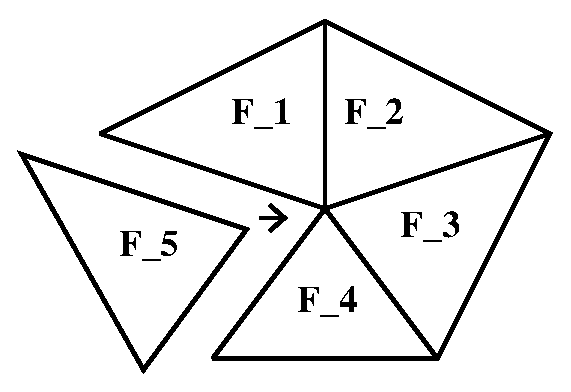
\includegraphics[totalheight=1in]{vic3fig1}
\end{center}

{\bf Obeservation 3:} $h_i(\Delta) =$ the number of factes in the shelling that have $i$ 
"old" walls and $d-i$ "new" walls.


{\bf Corollary 1:} For $\Delta$ shellable, $h_i(\Delta) \geq 0$ for all $i$.

{\bf Corollary 2:} For $\Delta$ the boundary of a \emph{simplicial} convex 
$d$-polytope, one has $h_i(\Delta) = h_{d-i}(\Delta)$ for all $i$.

(Note: These are the Dehn (1905) - Sommerville (1927) Equations. The 
original proof was topological. $h_0 = h_d$ is just Euler's formula, 
since $h_d$ is, up to a sign, the Euler characteristic.)

{\bf Proof of Corollary 2:} The reverse of a Brugesser-Mani shelling is also a shelling, with 
the notions of "old" and "new" walls reversed.

(Note: An arbitrary convex polytope can always be made simplicial by 
triangulating the non-simplicial faces. This just adds more faces.)

{\bf Question:} What about simplicial spheres that are not necessarily polytopal?

We can try to interpret $h_i(\Delta)$ differently, using $k[\Delta]$.

\newpage

{\bf Example:}

\begin{center}
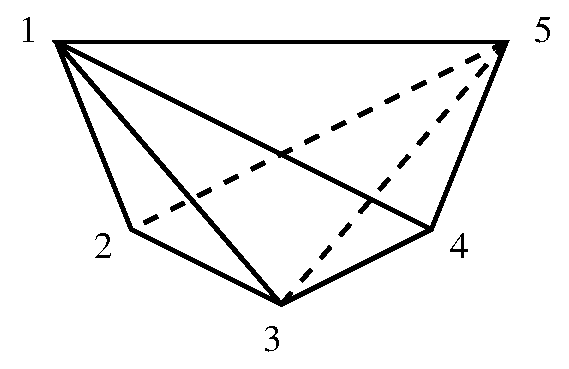
\includegraphics[totalheight=1in]{vic3fig2}
\end{center}

The maximal non-faces are $x_1 x_3 x_5$ and $x_2 x_4$, so
$$R = k[x_1, x_2, x_3, x_4, x_5]/(x_1 x_3 x_5, x_2 x_4)$$

(note that $R$ has Krull dimension 3), and 

$$Hilb(R,t) = \frac{1 + 2t + 2t^2 + t^3}{(1 - t)^3}.$$

It turns out that the three linear forms

\begin{center}
\begin{tabular}{l}
$\Theta_1 = x_3 - x_1$ \\
$\Theta_2 = x_5 - x_1$ \\
$\Theta_3 = x_4 - x_2$ \\
\end{tabular}
\end{center}

form an $R$-regular sequence, i.e.,

\begin{center}
\begin{tabular}{l}
$\Theta_1$ is a non zero-divisor of $R$, \\
$\Theta_2$ is a non zero-divisor of $R/(\Theta_1)$, \\
$\Theta_3$ is a non zero-divisor of $R/(\Theta_1, \Theta_2)$. \\
\end{tabular}
\end{center}

So
\begin{eqnarray}
R/(\Theta) & := & R/(\Theta_1, \Theta_2, \Theta_3) \nonumber \\
& = & K[x_1, x_2, x_3, x_4, x_5]/(x_1 x_3 x_5, x_2 x_4, x_3 - x_1, x_5 - 
x_1, x_4 - x_2) \nonumber \\
& = & k[y_1, y_2]/(y_1^3, y_2^2) \textrm{, where } y_1 = x_1, y_2 = x_2 \nonumber \\
& = & k \textrm{-span of } \{1, y_1, y_2, y_1^2, y_1 y_2, y_1^2 y_2 \}. \nonumber
\end{eqnarray}

Note that the basis has one element of degree 0, two of degree 1, two of 
degree 2 and one of degree 3. This matches the $h$-vector $h(\Delta) = 
(1, 2, 2, 1)$ we computed earlier. This is not a coincidence!


{\bf Fact:} If $R$ is a graded ring and $\Theta$ a homogeneous non zero-divisor of 
degree $m$, then
$$\textrm{Hilb}(R/(\Theta),t) = (1 - t^m)\textrm{Hilb}(R,t).$$

(Note: In our example, $m=1$ and we performed this process three times, to get 
$(1-t)^3 \frac{1 + 2t + 2t^2 + t^3}{(1-t)^3} = 1 + 2t + 2t^2 + t^3$.)

{\bf Reason:} Multiplication by $\Theta$ gives us a short exact sequence
$$0 \rightarrow R(-m) \rightarrow R \rightarrow R/(\Theta) \rightarrow 0.$$

($R(-m)$ is a free $R$-module whose basis element is degree $m$.)

The corresponding Hilbert series are $t^m \textrm{Hilb}(R,t)$, $\textrm{Hilb}(R,t)$, and 
$\textrm{Hilb}(R/(\Theta),t)$, and by exactness we get
$$t^m \textrm{Hilb}(R,t) - \textrm{Hilb}(R,t) + \textrm{Hilb}(R/(\Theta),t) = 0.$$

{\bf Definition:} A finitely generated $k$-algebra $R$ of Krull dimension $d$ 
is \emph{Cohen-Macaulay} (CM) if there exists an $R$-regular sequence 
$\Theta_1, \Theta_2, \ldots, \Theta_d$.

{\bf Fact 1:} If $R$ is CM and generated by elements of degree 1 (this is the case 
for a SR ring) then one can always choose $\Theta_1, \Theta_2, \ldots, 
\Theta_d$ of degree 1, as long as $k$ is "big enough" (which we can 
ensure by enlarging $k$ to $|k| = \infty$ without changing the 
characteristic).

Note: This is similar to Noether Normalization, but stronger.

Note: In a CM ring, \emph{every} system of parameters is a regular 
sequence.

{\bf Fact 2 (Reisner's Theorem, Minnesota PhD thesis, 1976):} For $\Delta$ a $d$-dimensional 
complex, $k[\Delta]$ is CM if and only if 
for every face $F$ of $\Delta$, the link has no reduced homology below 
dimension $d-1-\textrm{dim}F$, i.e., if and only if $H_i(\textrm{link}_\Delta(F); k) = 0$ for 
$i < 
d-1-\textrm{dim}F$. By Munkries, this happens if and only if $H_i(||\Delta||;k) = 0$ 
for $i < d$, which is if and only if $H_i(||\Delta||, ||\Delta|| - x) = 0$ for $i 
< d$ and all $x \in ||\Delta||$.

Note: The "star" of a face $F$ is a neighborhood of 
$F$. The link is the set of all faces disjoint from $F$, i.e., the base 
of the star.

\begin{center}
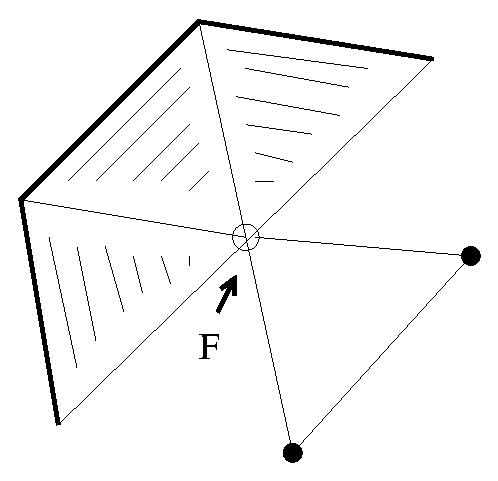
\includegraphics[totalheight=1in]{vic3fig3}
\end{center}

{\bf Corollary 1:} $\Delta$ a simplicial sphere implies $k[\Delta]$ is CM for 
all fields $k$

{\bf Corollary 2 (UBC for spheres, Stanley, 1975):} $\Delta$ a CM simplicial 
complex implies
$$0 \leq h_i(\Delta) \leq {{n-d+i-1}\choose{i}}.$$

{\bf Proof of Corollary 2:} $h_i(\Delta) = dim_k(R/(\Theta))_i$, so the quotient ring is 
isomorphic to a polynomial ring in $n-d$ variables quotient by 
some ideal. Hence $h_i(\Delta) \leq \textrm{dim}_k(k[y_1, y_2. \ldots, y_{n-d}]_i) 
= {{n-d+i-1}\choose{i}}$ (the number of monomials of degree $i$ from 
$n-d$ variables).

{\bf Example of a non-CM complex:}

\begin{center}
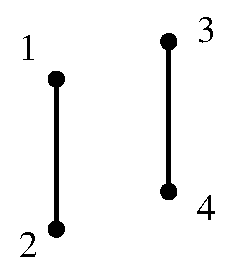
\includegraphics[totalheight=1in]{vic3fig4}
\end{center}

$$f = (f_{-1}, f_0, f_1) = (1, 4, 2)$$
$$h = (h_0, h_1, h_2) = (1, 2, -1)$$

Set $R = k[x_1, x_2, x_3, x_4]/(x_1 x_3, x_1 x_4, x_2 x_3, x_2 x_4)$. 
We can find one non zero-divisor, say $x_1 - x_3$, and quotient by $x_1 
- x_3$ to get $k[x_1, x_2, x_4]/(x_1^2, x_1 x_4, x_1 x_2, x_2 x_4)$. This 
ring has no non zero-divisors since, for example, everything of positive degree kills $x_1$.

Note: In this example $R$ is the coordinate ring of two 2-dimensional 
hyperplanes in 4-space, meeting at a single point. It is a standard 
example of a non-CM variety with equidimensionality. See Eisenbud's 
book.



\end{document}

